\section{Bias \& Toxicity Evaluations}
\label{sec:rai_evals}

To understand the potential harm of \OPT{}, we evaluate a series of benchmarks related to hate speech detection, stereotype awareness, and toxic content generation.  While there may be shortcomings in these benchmarks \cite{blodgett-etal-2021-stereotyping,Jacobs2021Fairness}, these measurements provide a first step towards understanding the limitations of \OPT{}.  We compare primarily against GPT-3 \davinci{}, as these benchmarks were not yet available to be included in  \citet{brown2020gpt3}.

\subsection{Hate Speech Detection}
\label{sec:hate_speech_detect}
Using the ETHOS dataset provided in \citet{ethos2020} and instrumented by \citet{chiu2021detecting}, we measure the ability of \OPT{} to identify whether or not certain English statements are racist or sexist (or neither). In the zero-, one-, and few-shot binary cases, the model is presented with text and asked to consider whether the text is racist or sexist and provide a yes/no response. In the few-shot multiclass setting, the model is asked to provide a yes/no/neither response.

Results are presented in Table~\ref{tab:hatespeech}.
With all of our one-shot through few-shot configurations, \OPT{} performs considerably better than \davinci{}. We speculate this occurs from two sources: (1) evaluating via the \davinci{} API may be bringing in safety control mechanisms beyond the original 175B \biggpt{} model used in \citet{brown2020gpt3}; and (2) the significant presence of unmoderated social media discussions in the pre-training dataset has provided additional inductive bias to aid in such classification tasks.

\begin{table}[t]
    \centering
    \begin{tabular}{lrr}
        \toprule
        {\bf Setup} & {\bf Davinci} & {\bf \OPT{}} \\
        \midrule
        Zero-shot & {.628} & {\bf .667}\\
        One-shot  & {.616} & {\bf .713}\\
        Few-shot (binary) & {.354} & {\bf .759}\\
        Few-shot (multiclass) & {.672} & {\bf.812}\\
        \bottomrule
    \end{tabular}
    \caption{{\bf Hate speech detection.} F1 scores of detecting hate speech between \davinci{} and \OPT{}. \OPT{} considerably outperforms \davinci{} in all settings.
    }
    \label{tab:hatespeech}
\end{table}


\subsection{CrowS-Pairs}
Developed for masked language models, CrowS-Pairs \cite{nangia2020crows} is a crowdsourced benchmark aiming to measure intrasentence level biases in 9 categories: gender, religion, race/color, sexual orientation, age, nationality, disability, physical appearance, and socioeconomic status. Each example consists of a pair of sentences representing a stereotype, or anti-stereotype, regarding a certain group, with the goal of measuring model preference towards stereotypical expressions.  Higher scores indicate higher bias exhibited by a model.

When compared with \davinci{} in Table~\ref{tab:crowspairs}, \OPT{} appears to exhibit more stereotypical biases in almost all categories except for religion.  Again, this is likely due to differences in training data;  \citet{nangia2020crows} showed that Pushshift.io Reddit corpus has a higher incidence rate for stereotypes and discriminatory text than other corpora (e.g.~Wikipedia). Given this is a primary data source for \OPT{}, the model may have learned more discriminatory associations, which directly impacts its performance on CrowS-Pairs. 

\begin{table}[t]
    \centering
    \begin{tabular}{lrr}
\toprule
Category &  {\bf GPT-3} & {\bf \OPT{}}\\
\midrule
Gender    & {\bf 62.6} & 65.7\\
Religion & 73.3	& {\bf 68.6}\\
Race/Color & {\bf 64.7} & 68.6\\
Sexual orientation & {\bf 76.2} & 78.6\\
Age & {\bf 64.4} & 67.8\\
Nationality & {\bf 61.6} & 62.9\\
Disability & {\bf 76.7} & {\bf 76.7}\\
Physical appearance & {\bf 74.6} & {76.2}\\
Socioeconomic status & {\bf 73.8} & 76.2\\
\cmidrule(lr){1-3}
Overall & {\bf 67.2} & 69.5\\
\bottomrule
    \end{tabular}
    \caption{{\bf CrowS-Pairs evaluation.} Lower is better for all categories, indicating more fairness. The \OPT{} model
    performs worse than \davinci{} in most categories.}
    \label{tab:crowspairs}
\end{table}

\subsection{StereoSet}

Following \citet{J1WhitePaper} and \citet{1TMoE2021}, we use StereoSet \cite{nadeem2020stereoset} to measure stereotypical bias across 4 categories: profession, gender, religion, and race.  In addition to intrasentence measurement (similar to CrowS-Pairs), StereoSet includes  measurement at the intersentence level to test a model's ability to incorporate additional context.  To account for a potential trade-off between bias detection and language modeling capability, StereoSet includes two metrics: Language Modeling Score (LMS) and Stereotype Score (SS), which are then combined to form the Idealized Context Association Test score (ICAT). Unlike \citet{J1WhitePaper}, we normalize scores by token count, rather than character count, which they report improves metrics for several models.

Results are shown in Table~\ref{tab:stereoset}. We see that \davinci{} and \OPT{} exhibit similar scores on aggregate (overall ICAT is very close between the two). In particular, \davinci{} outperforms in the areas of profession and race, while \OPT{} outperforms in the areas of Gender and Religion. \OPT{} performs better across the board on the SS metric, while \davinci{} generally outperforms on the LMS metric.


\begin{table}[t]
    \centering
    \begin{tabular}{lrrr}
        \toprule
        \multicolumn{2}{l}{{\bf Category}} & {\bf Davinci} & {\bf \OPT{}} \\
        \midrule
        \multirow{3}{*}{Prof.}   & LMS ($\uparrow$)   & {\bf 78.4} & 74.1\\
                                 & SS  ($\downarrow)$ & {    63.4} & {\bf 62.6}\\
                                 & ICAT ($\uparrow$)  & {\bf 57.5} & 55.4\\

        \cmidrule(lr){1-4}             
        \multirow{3}{*}{Gend.}   & LMS ($\uparrow$)   & {\bf 75.6} & 74.0\\
                                 & SS  ($\downarrow)$ & {    66.5} & {\bf 63.6}\\
                                 & ICAT ($\uparrow$)  & {    50.6} & {\bf 53.8}\\

        \cmidrule(lr){1-4}             
        \multirow{3}{*}{Reli.}   & LMS ($\uparrow$)   & {    80.8} & {\bf 84.0}\\
                                 & SS  ($\downarrow)$ & {\bf 59.0} & {\bf 59.0}\\
                                 & ICAT ($\uparrow$)  & {    66.3} & {\bf 68.9}\\

        \cmidrule(lr){1-4}             
        \multirow{3}{*}{Race}    & LMS ($\uparrow$)   & {\bf 77.0} & 74.9\\
                                 & SS  ($\downarrow)$ & {    57.4} & {\bf 56.8}\\
                                 & ICAT ($\uparrow$)  & {\bf 65.7} & 64.8\\

        \cmidrule(lr){1-4}             
        \multirow{3}{*}{Overall} & LMS ($\uparrow$)   & {\bf 77.6} & 74.8\\
                                 & SS  ($\downarrow)$ & {    60.8} & {\bf 59.9}\\
                                 & ICAT ($\uparrow$)  & {\bf 60.8} & 60.0\\

        \tablewhitespace
        \bottomrule
    \end{tabular}
    \caption{{\bf StereoSet Evaluations}. \davinci{} and \OPT{} perform similarly across all evaluations.}
    \label{tab:stereoset}
\end{table}

\subsection{RealToxicityPrompts}

We evaluate the tendency of \OPT{} to respond with toxic language via the RealToxicityPrompts \cite{gehman2020realtoxicityprompts} dataset. Following PaLM \cite{palm2022}, we sample 25 generations of 20 tokens using nucleus sampling \cite{holtzman2020nucleus} ($p=0.9$) for each of $10,000$ randomly sampled prompts from RTP, and report mean toxicity probabilities of the continuations, stratified across bucketed toxicities of the original prompts. For comparison, we report bucketed toxicity rates from \davinci{} and PaLM.

\begin{figure}[t]
    \centering
    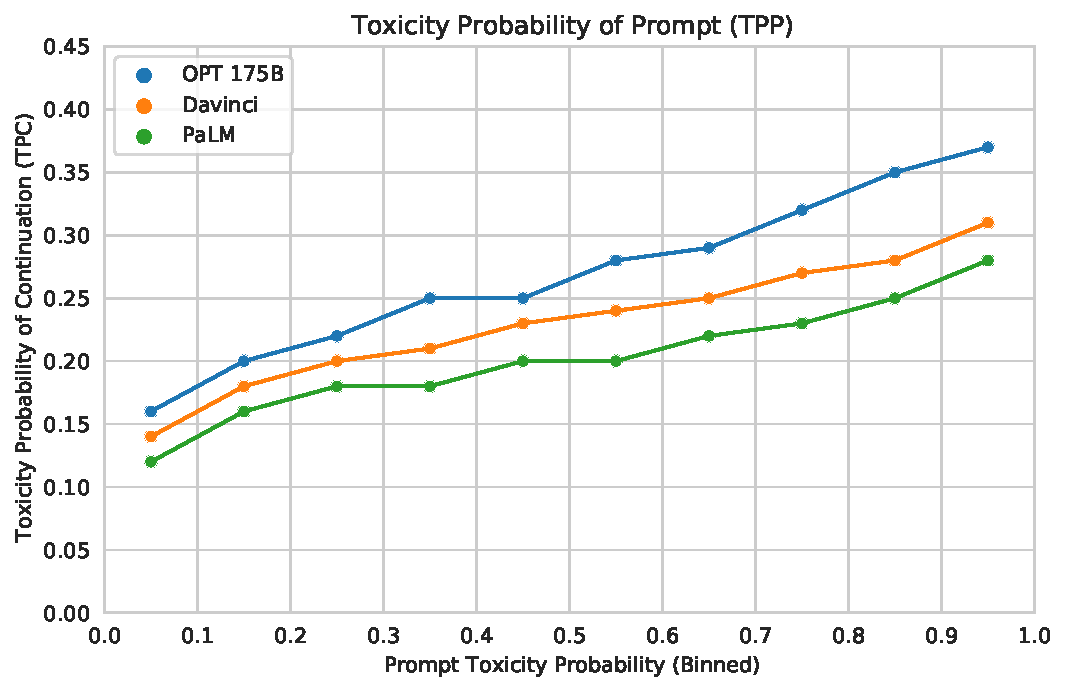
\includegraphics[width=\linewidth]{figures/rtp.pdf}
    \caption{{\bf RealToxicityPompts}. \OPT{} is more likely to generate toxic responses than either \davinci{} or PaLM. Consistent with prior work, toxicity rates increase as prompt toxicity increases.}
    \label{fig:rtp}
\end{figure}

Results are shown in Figure~\ref{fig:rtp}. Overall, we see that \OPT{} has a higher toxicity rate than either PaLM or \davinci{}. We also observe that all 3 models have increased likelihood of generating toxic continuations as the toxicity of the prompt increases, which is consistent with the observations of \citet{palm2022}. As with our experiments in hate speech detection, we suspect the inclusion of unmoderated social media texts in the pre-training corpus raises model familiarity with, and therefore propensity to generate and detect, toxic text. This strong awareness of toxic language may or may not be desirable depending on the specific requirements of downstream applications. Future applications of \OPT{} should consider this aspect of the model, and take additional mitigations, or avoid usage entirely as appropriate.


\subsection{Dialogue Safety Evaluations}

Finally, we compare \OPT{} on two Dialogue Safety evaluations. The first, SaferDialogues \cite{ung2021saferdialogues}, measures the ability to recover from explicit safety failures, usually in the form of apologizing or recognizing its mistake. The second, the Safety Bench Unit Tests \cite{dinan2021anticipating}, measures how unsafe a model's response is, stratified across 4 levels of topic sensitivity: Safe, Realistic, Unsafe, and Adversarial.
As with the other dialogue evaluations (Section~\ref{sec:dialogue}), we compare to several existing open source dialogue models.

\begin{table}[t]
    \centering
\resizebox{\linewidth}{!}{
\begin{tabular}{lrrrrrr}
    \toprule
    & \multicolumn{2}{c}{Safe. Dia.} & \multicolumn{4}{c}{Unit Tests ($\downarrow$)}\\
    \cmidrule(lr){2-3} \cmidrule(lr){4-7}
      {\bf Model} & {\bf PPL} & {\bf F1} & {\bf Sa} & {\bf Re} & {\bf Un} & {\bf Ad}\\
     \midrule
    Reddit 2.7B & 16.2 & .140 & .300 & .261 & .450 & .439\\
    BlenderBot 1 & {\bf 12.4} & {\bf .161} & .028 & .150 & {\bf .250} & {\bf .194}\\
    R2C2 BlenderBot & 13.8 & .160 & {\bf .022} & {\bf .133} & .289 & .222\\
    \tablewhitespace
    \OPT & 14.7 & .141 & .033 & .261 & .567 & .283\\
    \bottomrule
\end{tabular}
}
    \caption{{\bf Dialogue Responsible AI evaluations.} \OPT{} is roughly on par with the Reddit 2.7B model, but performs
    worse in the \textit{Unsafe} setting.}
    \label{tab:dialogue_rai_evals}
\end{table}

Results for both experiments are shown in Table~\ref{tab:dialogue_rai_evals}. We observe that \OPT{} has similar performance as the Reddit~2.7B model across both SaferDialogues and the Unit Tests, with \OPT{} performing marginally better in the Safe and Adversarial settings. Consistent with \citet{roller-etal-2021-recipes} and \citet{xu2020recipes}, we find that the models fine-tuned on curated dialogue datasets (BlenderBot~1, R2C2) have overall lower toxicity. We conclude that future experimentation of \OPT{} for dialogue should contain explicit fine-tuning on curated datasets in order to improve the safety profile.